\section{Build \& Run}
The installation and execution of each part of the system comprises two steps:

\begin{itemize}
   \item \texttt{build} --
   Basically, this step corresponds to the installation of the product.
   It is necessary to download and create all the docker
   images. Also, it generate the configuration files both for the simulator and
   Docker. Indeed, some Dockerfiles are generated starting from a template and
   instantiated based on the environment chosen by the user. This choice defines
   also which components will be inserted in the image. As future work,
   we might shift this decision at runtime and keep only a single image for each
   environment.
   \item \texttt{run} --
   This step requires Docker Swarm
	or Docker Compose depending on the configurations chosen for the build.
	We provide only the complete system configurations and not the
	configuration of each single component.
   However, during the development of the project,
	the system used to be run with the latter configuration.
	So, it would be straightforward to provide all the possible configuration.
	If you have chosen to configure the system as a whole, then Docker Swarm
   will deploy it as a composition of stacks:
   each stack is a set of services which represents
   a city. Note that a service is not necessarily a container.
   A service can represent a set of containers which are kept under the same
   name by Docker Swarm.
   Also, not all the stacks represents a city. Indeed, the AMQP broker
   and the viewer components are wrapped in a separated
   stack which is unique within the system (i.e., does not depend upon the
   number of cities). Wrapping up, we have a stack for each city because
   each city has a different number of districts which are mapped in different
   services plus a single stack for the front end.
   Note that the size of each city and the number of deployed
   cities remarkably affect the time required to complete the run process:
   the greater the number of cities, the longer it will take.
\end{itemize}

Figure \ref{fig:deploy-sys} exemplifies the deployment of an instance of the
system.

\begin{figure}[H]
\centering
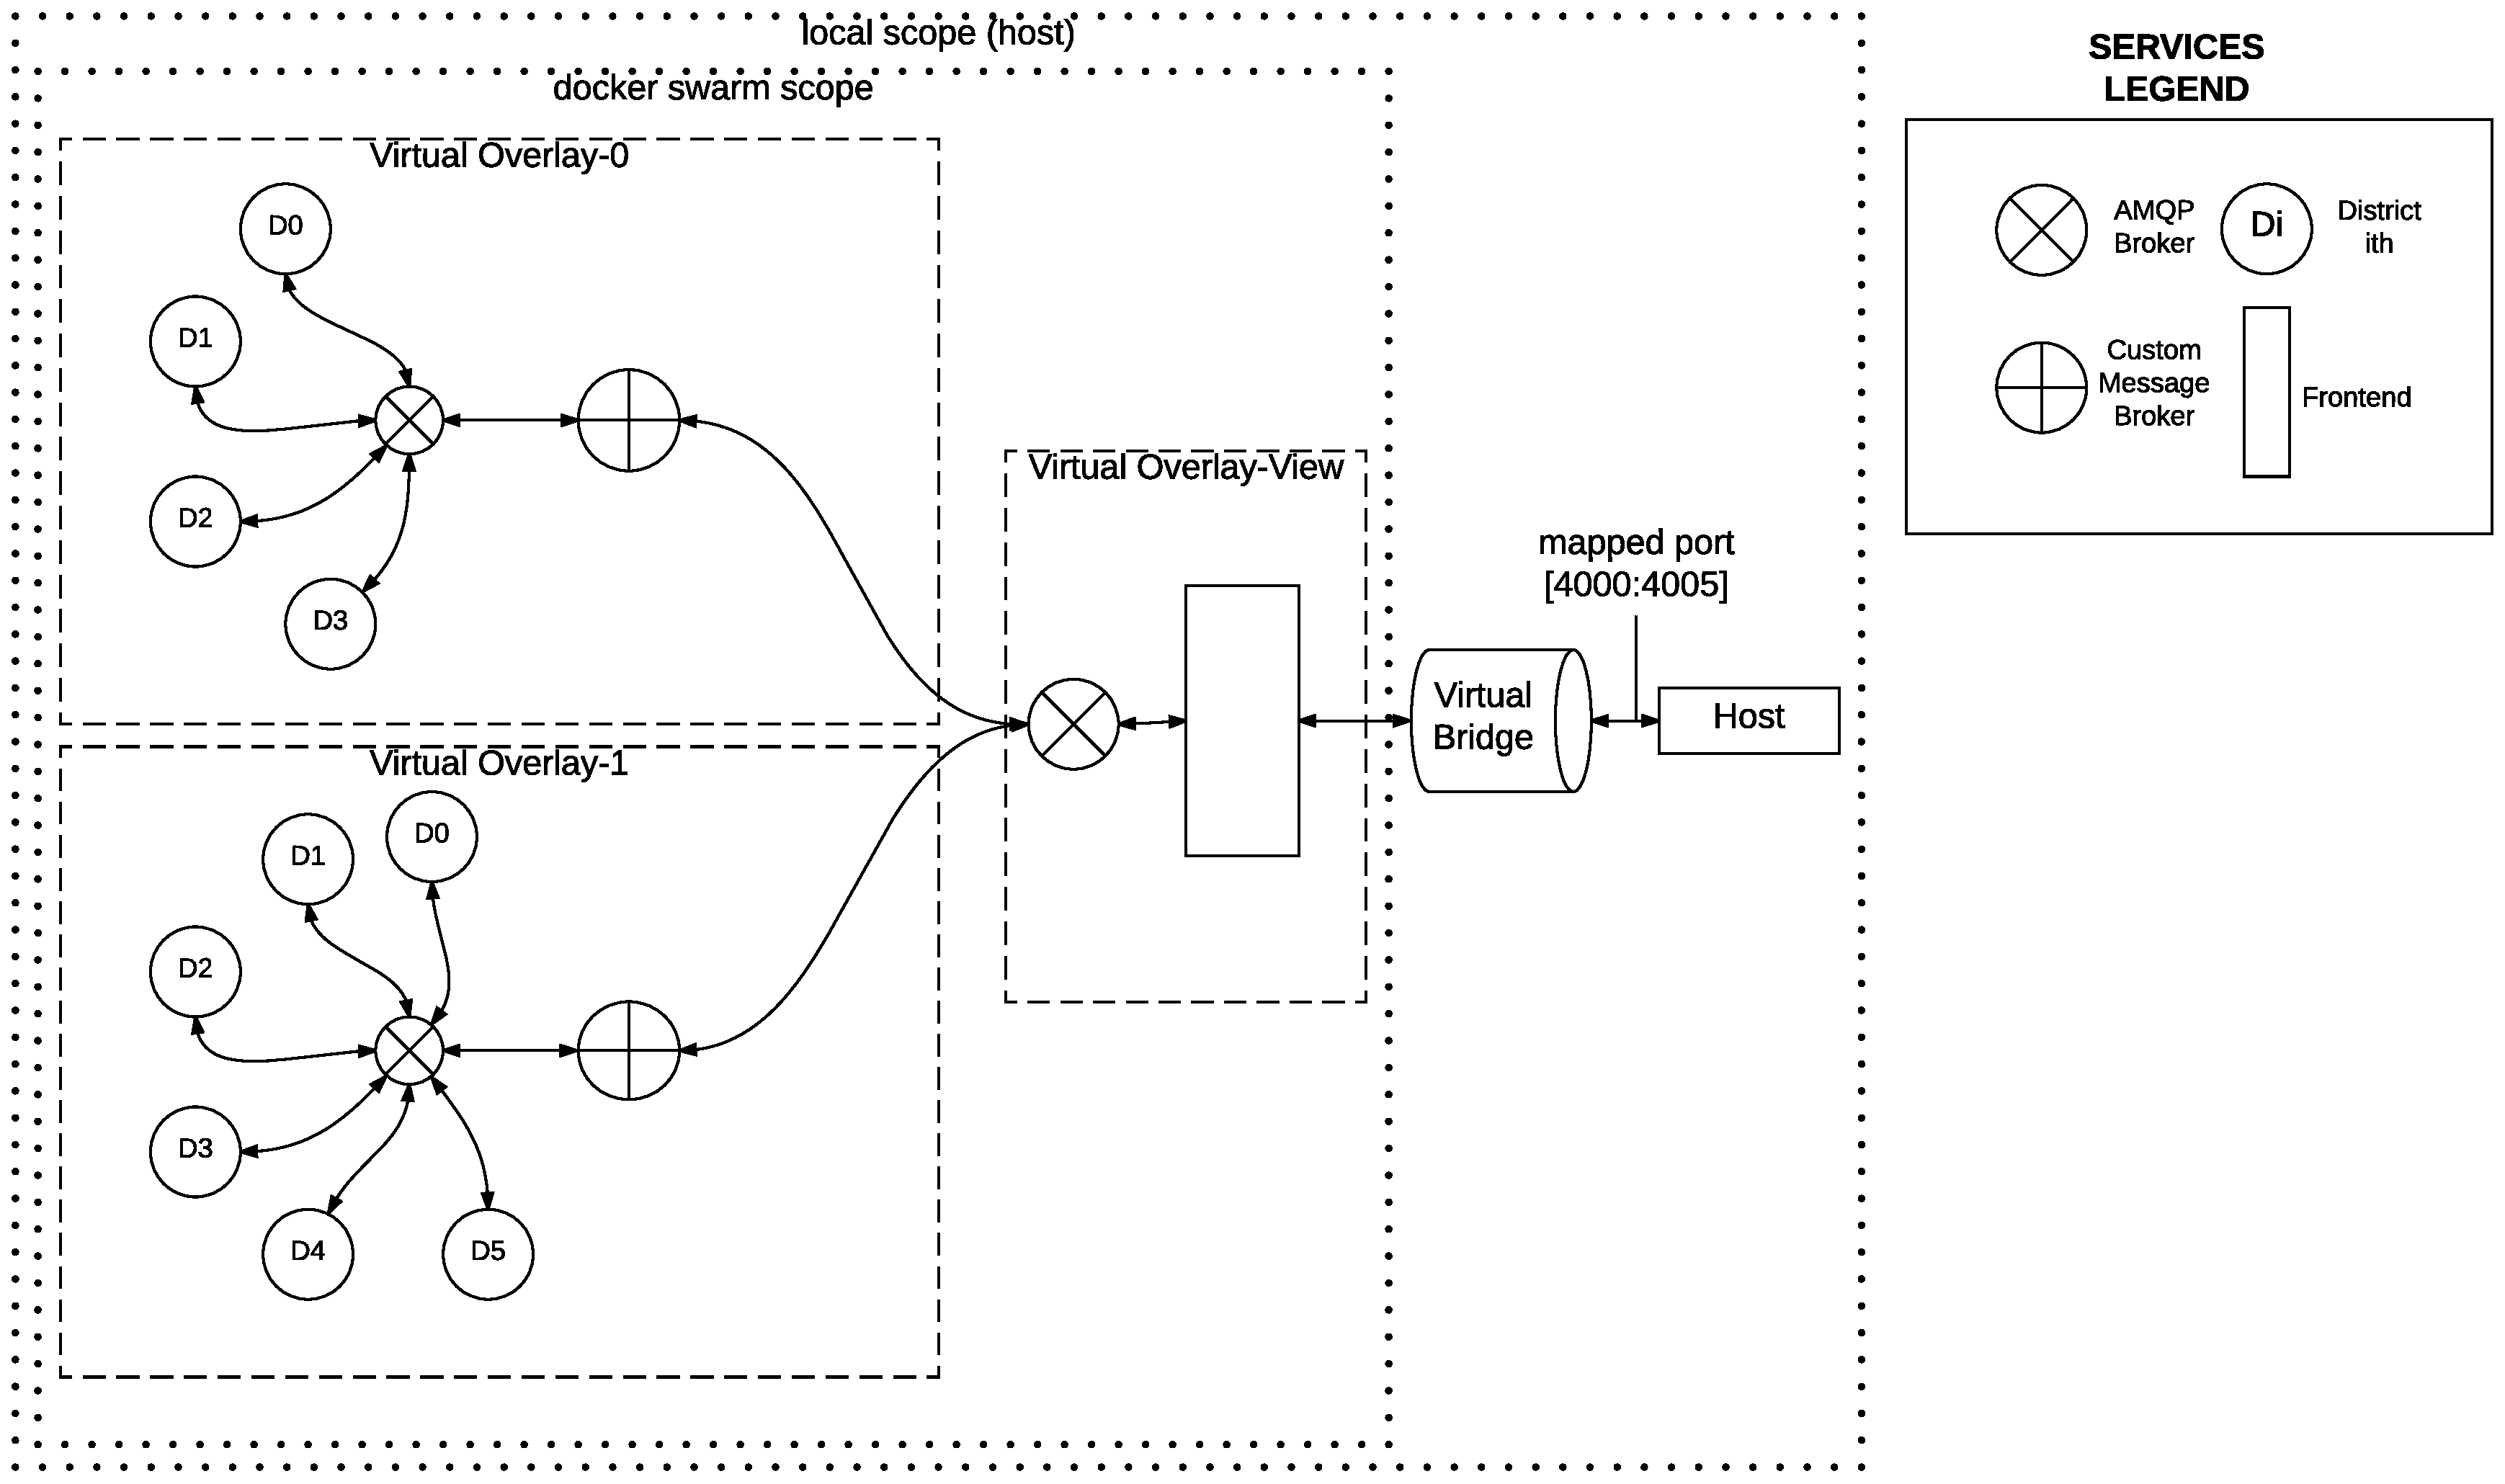
\includegraphics[scale=0.3,keepaspectratio]{images/user-man/eps/deploy.eps}
\caption{Example of a deployed ACTS system}
\label{fig:deploy-sys}
\end{figure}
